\documentclass[11pt, a4paper]{article}\usepackage[]{graphicx}\usepackage[]{color}
%% maxwidth is the original width if it is less than linewidth
%% otherwise use linewidth (to make sure the graphics do not exceed the margin)
\makeatletter
\def\maxwidth{ %
  \ifdim\Gin@nat@width>\linewidth
    \linewidth
  \else
    \Gin@nat@width
  \fi
}
\makeatother

\definecolor{fgcolor}{rgb}{0.345, 0.345, 0.345}
\newcommand{\hlnum}[1]{\textcolor[rgb]{0.686,0.059,0.569}{#1}}%
\newcommand{\hlstr}[1]{\textcolor[rgb]{0.192,0.494,0.8}{#1}}%
\newcommand{\hlcom}[1]{\textcolor[rgb]{0.678,0.584,0.686}{\textit{#1}}}%
\newcommand{\hlopt}[1]{\textcolor[rgb]{0,0,0}{#1}}%
\newcommand{\hlstd}[1]{\textcolor[rgb]{0.345,0.345,0.345}{#1}}%
\newcommand{\hlkwa}[1]{\textcolor[rgb]{0.161,0.373,0.58}{\textbf{#1}}}%
\newcommand{\hlkwb}[1]{\textcolor[rgb]{0.69,0.353,0.396}{#1}}%
\newcommand{\hlkwc}[1]{\textcolor[rgb]{0.333,0.667,0.333}{#1}}%
\newcommand{\hlkwd}[1]{\textcolor[rgb]{0.737,0.353,0.396}{\textbf{#1}}}%

\usepackage{framed}
\makeatletter
\newenvironment{kframe}{%
 \def\at@end@of@kframe{}%
 \ifinner\ifhmode%
  \def\at@end@of@kframe{\end{minipage}}%
  \begin{minipage}{\columnwidth}%
 \fi\fi%
 \def\FrameCommand##1{\hskip\@totalleftmargin \hskip-\fboxsep
 \colorbox{shadecolor}{##1}\hskip-\fboxsep
     % There is no \\@totalrightmargin, so:
     \hskip-\linewidth \hskip-\@totalleftmargin \hskip\columnwidth}%
 \MakeFramed {\advance\hsize-\width
   \@totalleftmargin\z@ \linewidth\hsize
   \@setminipage}}%
 {\par\unskip\endMakeFramed%
 \at@end@of@kframe}
\makeatother

\definecolor{shadecolor}{rgb}{.97, .97, .97}
\definecolor{messagecolor}{rgb}{0, 0, 0}
\definecolor{warningcolor}{rgb}{1, 0, 1}
\definecolor{errorcolor}{rgb}{1, 0, 0}
\newenvironment{knitrout}{}{} % an empty environment to be redefined in TeX

\usepackage{alltt} %or article has only section and below, book and report also have chapter: http://texblog.org/2007/07/09/documentclassbook-report-article-or-letter/

\usepackage[utf8]{inputenc}  % use utf8 encoding of symbols such as umlaute for maximal compatibility across platforms

\usepackage{caption}				% provides commands for handling caption sizes etc.
%\usepackage[a4paper, left=25mm, right=20mm, top=25mm, bottom=20mm]{geometry}		 % to easily change margin widths: https://www.sharelatex.com/learn/Page_size_and_margins

\usepackage{etoolbox}    % for conditional evaluations!
\usepackage[bottom]{footmisc}  % I love footnotes! And they should be down at the bottom of the page!
\usepackage{graphicx}        % when using figures and alike
\usepackage[hidelinks]{hyperref}		% for hyperreferences (links within the document: references, figures, tables, citations)

\usepackage{euler}     % a math font, only for equations and alike; call BEFORE changing the main font; alternatives: mathptmx, fourier, 
%\usepackage{gentium} % for a different font; you can also try: cantarell, charter, libertine, gentium, bera, ... http://tex.stackexchange.com/questions/59403/what-font-packages-are-installed-in-tex-live

%------------------------------------------------------------------------------------------------------
%------- text size settings --------------
\setlength{\textwidth}{16cm}% 
\setlength{\textheight}{25cm} %23 
%(these values were used to fill the page more fully and thus reduce the number of pages!)
\setlength{\topmargin}{-1.5cm} %0
\setlength{\footskip}{1cm} %
%\setlength{\hoffset}{0cm} %
\setlength{\oddsidemargin}{1cm}%
\setlength{\evensidemargin}{-.5cm}%
\setlength{\parskip}{0cm} % Abstand zwischen Absätzen
% ----------------------------------------------------------------
\renewcommand{\textfraction}{0.1} % allows more space to graphics in float
\renewcommand{\topfraction}{0.85}
%\renewcommand{\bottomfraction}{0.65}
\renewcommand{\floatpagefraction}{0.70}


\frenchspacing %http://texwelt.de/wissen/fragen/1154/was-ist-french-spacing-was-macht-frenchspacing
%------------------------------------------------------------------------------------------------------
%------------------------------------------------------------------------------------------------------
\IfFileExists{upquote.sty}{\usepackage{upquote}}{}
\begin{document}
\SweaveOpts{concordance=TRUE}
%\SweaveOpts{concordance=TRUE}
%%%%%%%%%%%%% this bit is new to Knitr: %%%%%%%%%%%%%%%%%%%%%



\title{A tutorial for Step Selection Function}

\author{P. Antkowiak\thanks{M.Sc. programme "GIS und Umweltmodellierung" at University of Freiburg} \and H. Tripke\thanks{M.Sc. programme "Wildlife, Biodiversity and Vegetation" at University of Freiburg} \and C. Wilhelm\thanks{M.Sc. programme "Wildlife, Biodiversity and Vegetation" at University of Freiburg}}
% for more control, multiple affiliations, line breaks and alike, use the authblk package!!

\date{\today} % !!use package isodate for more control of date formatting!!

\maketitle

%------------------------------------------------------------------------------------------------------
%------------------------------------------------------------------------------------------------------

\tableofcontents

\newpage

\section{Introduction}%------------------------------------------------------------------------------------------------------
In addition to Resources Selection Functions (RSF) a more detailed anlysis for telemetry data can be conducted by using Step Selection Function (SSF). The use of latter is providing answers to th actual selection of animals on their habitat rather than analysing the use of a habitat only. (DO WE WANT TO CITE, HERE FOR EXAMPLE Simone and friends). So far most of the SSF were done in GIS to use spatial data together with mathematics equations. However, more and more packages are provided in R and thus becomes a valuable alternative. \
This tutorial provides an overview on how to implement SSF with R. The main package we will use in the following is the package \textbf{adehabitatLT}. All single steps that need to be taken care of are summarized in (Figure~\ref{fig:Flowchart}).\
In our tutorial we use telemetry data from Cougars/Mountain Lion (\textit{Latin name}) collected by Simone Ciuti\footnote{we might have to specify that and name and thank the institute.../collected/containing}. As spatial parameters x tables for ruggedness, slope, canopy cover etc. are available. Describe study area...\
Why did we not use the data (Wildboar) prepared for the adehabitatLT package? - No information on details, metadata provided, it is hard to understand when to use which dataset and why.


\begin{figure} % you can (but shouldn't) use [h] behind {figure} to force the picture to go here. However, the idea of LaTeX is that it will do things for you, so too much interfering is not saving you any time.
% see also here: http://en.wikibooks.org/wiki/LaTeX/Floats,_Figures_and_Captions#Captions
\captionsetup{width=0.8\textwidth}
\centering
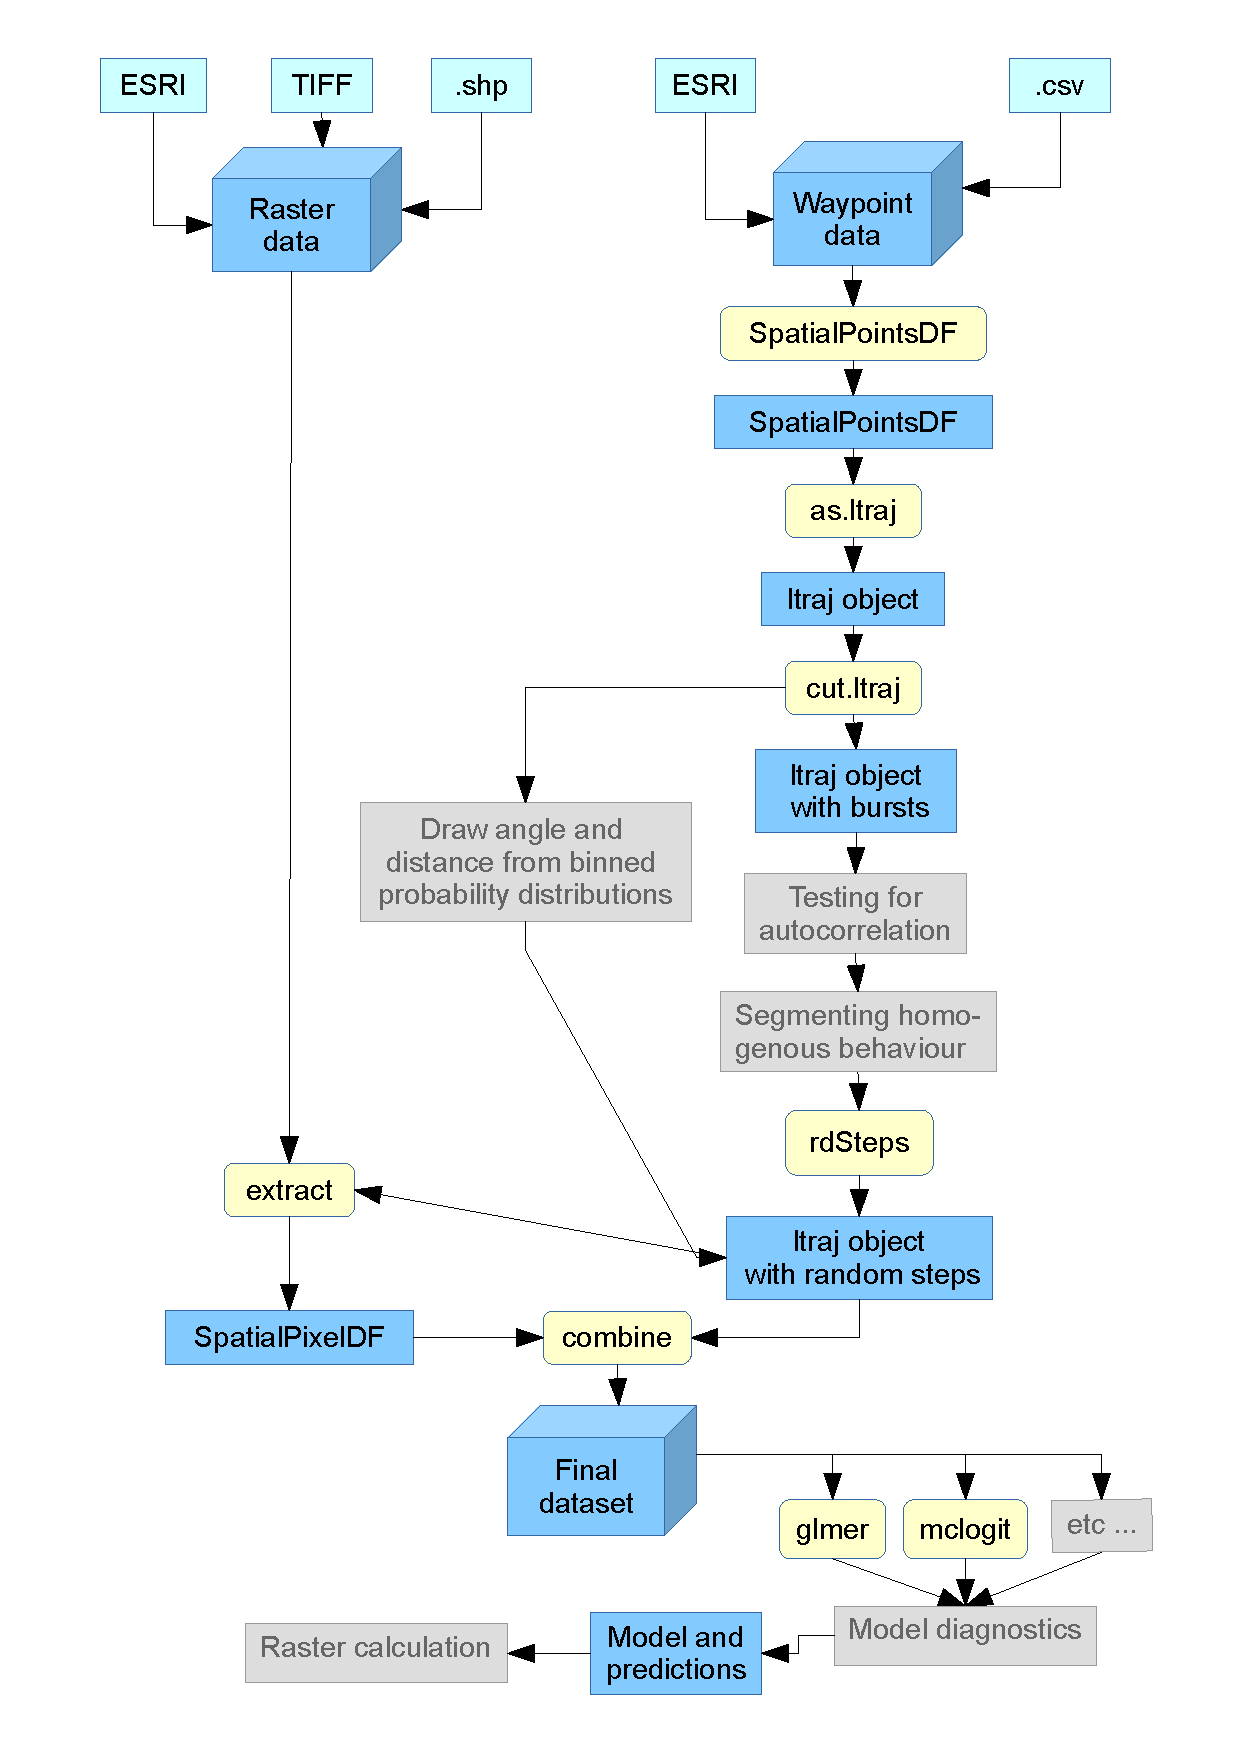
\includegraphics[width=0.8\textwidth]{Flowchart.pdf} %our perfect workflow!
\caption{\emph{Conducting a SSF using existing R-packages:} this figures provides an overview of the steps necessary to conduct a SSF. The steps are separated in subsections, which the turtorial will guide you through.}
\label{fig:Flowchart}
\end{figure}




\section{Preparations}
Before you can actually start using the tutorial for conducting SSF you need to load a bunch of packages in R. Some of them require others so that you have to add all these to your library:

\subsection{Packages - what we need}

\begin{knitrout}
\definecolor{shadecolor}{rgb}{0.969, 0.969, 0.969}\color{fgcolor}\begin{kframe}
\begin{alltt}
\hlcom{# installing packages -----------------------------------------------------}
\hlcom{## for implementing SSF}
\hlcom{# install.packages("adehabitat") # outdated version, not needed for this tutorial}
\hlkwd{install.packages}\hlstd{(}\hlstr{"adehabitatHR"}\hlstd{)}
\hlkwd{install.packages}\hlstd{(}\hlstr{"adehabitatHS"}\hlstd{)}
\hlkwd{install.packages}\hlstd{(}\hlstr{"adehabitatLT"}\hlstd{)}
\hlkwd{install.packages}\hlstd{(}\hlstr{"adehabitatMA"}\hlstd{)}
\hlkwd{install.packages}\hlstd{(}\hlstr{"tkrplot"}\hlstd{)}
\hlkwd{install.packages}\hlstd{(}\hlstr{"hab"}\hlstd{,} \hlkwc{repos} \hlstd{=} \hlstr{"http://ase-research.org/R/"}\hlstd{)} \hlcom{# regular}
\hlkwd{install.packages}\hlstd{(}\hlstr{"hab"}\hlstd{,} \hlkwc{repos} \hlstd{=} \hlstr{"http://ase-research.org/R/"}\hlstd{,} \hlkwc{type} \hlstd{=} \hlstr{"source"}\hlstd{)} \hlcom{# for self-compiling}

\hlcom{# for handling ratser data}
\hlkwd{install.packages}\hlstd{(}\hlstr{"move"}\hlstd{)}
\hlkwd{install.packages}\hlstd{(}\hlstr{"raster"}\hlstd{)}
\hlkwd{install.packages}\hlstd{(}\hlstr{"rgdal"}\hlstd{)}
\hlcom{#install.packages("")}

\hlcom{# loading the packages}
\hlcom{# require(adehabitat) # keep fingers off this package. It is outdated.}
\hlkwd{require}\hlstd{(hab)}
\hlkwd{require}\hlstd{(adehabitatMA)}
\hlkwd{require}\hlstd{(adehabitatHR)}
\hlkwd{require}\hlstd{(adehabitatHS)}
\hlkwd{require}\hlstd{(adehabitatLT)}

\hlcom{## for i dont know}

\hlcom{#require(move)}
\hlcom{#require(raster)}
\hlcom{#require(rgdal)}
\hlcom{#require(tkrplot)}
\hlcom{#require(raster)}
\hlcom{#require(sp)}
\end{alltt}
\end{kframe}
\end{knitrout}

\section{Spatial covariates}%----------------------------------------------------------------------------------------------------------------------------
This section explains the use of spatial parameters that will be tested for selection by the target species. You should store these data in raster files (probably ESRI (*.adf) or *.tif) and for time reasons already clipped to your area. How you can do this in R please read the GIS instructions from the other group ;)   

\subsection{Load raster data (ESRI, *.tif, (*.shp))}%------------------------------------------------------------------------------------------------------
With a simple function stored in the package \textbf{raster} you are able to upload any ratser file into R. Examplarily we are using the ratser data for ruggedness and canopy cover for the study area.  


\begin{knitrout}
\definecolor{shadecolor}{rgb}{0.969, 0.969, 0.969}\color{fgcolor}\begin{kframe}
\begin{alltt}
\hlcom{#install.packages("RArcInfo")}
\hlcom{#require(RArcInfo)}
\hlkwd{require}\hlstd{(raster)}
\hlkwd{require}\hlstd{(rgdal)}

\hlkwd{require}\hlstd{(sp)}


\hlcom{#?raster}
\hlcom{#getwd()}
\hlcom{#setwd("/home/Peter/")}

\hlstd{ruggedness} \hlkwb{<-} \hlkwd{raster}\hlstd{(}\hlstr{"/home/Peter/Dokumente/uni/WS_14_15/Best Practice R/Dataset/NEW GIS LAYERS/tri1/w001001.adf"}\hlstd{)}
\hlcom{# plot(ruggedness) # outcomment this if you just quickly want to run the script. Takes a minute to process.}

\hlstd{landcover} \hlkwb{<-} \hlkwd{raster}\hlstd{(}\hlstr{"/home/Peter/Dokumente/uni/WS_14_15/Best Practice R/Dataset/NEW GIS LAYERS/lc_30/w001001.adf"}\hlstd{)}
\hlcom{# plot(landcover) # outcomment this if you just quickly want to run the script. Takes a minute to process.}

\hlstd{canopycover} \hlkwb{<-} \hlkwd{raster}\hlstd{(}\hlstr{"/home/Peter/Dokumente/uni/WS_14_15/Best Practice R/Dataset/NEW GIS LAYERS/cc_abmt/w001001.adf"}\hlstd{)}
\hlcom{# plot(canopycover) # outcomment this if you just quickly want to run the script. Takes a minute to process.}

\hlstd{disthighway} \hlkwb{<-} \hlkwd{raster}\hlstd{(}\hlstr{"/home/Peter/Dokumente/uni/WS_14_15/Best Practice R/Dataset/NEW GIS LAYERS/disthwy/w001001.adf"}\hlstd{)}
\hlcom{# plot(disthighway) # outcomment this if you just quickly want to run the script. Takes a minute to process.}

\hlstd{distroad} \hlkwb{<-} \hlkwd{raster}\hlstd{(}\hlstr{"/home/Peter/Dokumente/uni/WS_14_15/Best Practice R/Dataset/NEW GIS LAYERS/distsmrd/w001001.adf"}\hlstd{)}
\hlkwd{plot}\hlstd{(distroad)} \hlcom{# outcomment this if you just quickly want to run the script. Takes a minute to process.}
\end{alltt}
\end{kframe}
\end{knitrout}


\subsection{Extract coordinates for comparison of used and random points} %------------------------------------------------------------------------------------------------------
Peter is successfully doing this step!!

\section{Load telemetry data (*.csv, ESRI)}%------------------------------------------------------------------------------------------------------
The data for the analysis should be safed in a simple *.csv format. Depending on your analysis you have to include 
\begin{enumerate}
\item{ID}
\item{coordinates}
\item{date and/or time}
\item{...}
\end{enumerate}



\section{Create a Spatial Points Data Frame}%------------------------------------------------------------------------------------------------------

\section{Create a ltraj object}%------------------------------------------------------------------------------------------------------


\section{Creating Bursts}%

For analysing the data, there might be the need to create "sub-bursts" within your trajectory. For example, if the individuals were only recorded during the day, the monitoring took place over two consecutive years or the time lag between the relocations differs remarkably. Looking at those different parts seperately might be necessary for different reasons. The function \texttt{cutltraj} splits the given bursts of your \texttt{ltraj} object into smaller burst according to a specified criterion. In contrast, the function \texttt{bindltraj} combines the bursts of an object of class \texttt{ltraj} with the same attribute "id" to one unique burst. (c. Calenge) To find out if there are more missing values, you can plot the \texttt{ltraj} object. For that, you need to define the time interval you are looking at. 


In our example, the locations of the cougars were recorded every 3 hours, starting at 3 AM. The location at midnight is always missing. We now want to split the existing bursts (individuals) into "sub-bursts" where the time lag is smaller than 3 hours. To get an impression about the time lags we plotted the different bursts (individuals).

\begin{knitrout}
\definecolor{shadecolor}{rgb}{0.969, 0.969, 0.969}\color{fgcolor}\begin{kframe}
\begin{alltt}
\hlkwd{plotltr}\hlstd{(xmpl.ltr,} \hlstr{"dt/3600"}\hlstd{)}
\hlkwd{plotltr}\hlstd{(xmpl.ltr,} \hlstr{"dt/3600/3"}\hlstd{)}
\end{alltt}
\end{kframe}
\end{knitrout}

Because we want to keep relocations which are only a few minutes "wrong", we need a function which defines \texttt{dt}, which is the time interval between successive relocations (measured in seconds).

\begin{knitrout}
\definecolor{shadecolor}{rgb}{0.969, 0.969, 0.969}\color{fgcolor}\begin{kframe}
\begin{alltt}
\hlstd{foo} \hlkwb{=} \hlkwa{function}\hlstd{(}\hlkwc{dt}\hlstd{) \{}\hlkwd{return}\hlstd{(dt}\hlopt{>} \hlstd{(}\hlnum{3800}\hlopt{*}\hlnum{3}\hlstd{))\}}
\end{alltt}
\end{kframe}
\end{knitrout}

Then we split the object of class \texttt{ltraj} according to that function into smaller bursts. The bursts we had before applying this function still remain.

\begin{knitrout}
\definecolor{shadecolor}{rgb}{0.969, 0.969, 0.969}\color{fgcolor}\begin{kframe}
\begin{alltt}
\hlstd{xmpl.cut} \hlkwb{<-} \hlkwd{cutltraj}\hlstd{(xmpl.ltr,} \hlstr{"foo(dt)"}\hlstd{,} \hlkwc{nextr} \hlstd{=} \hlnum{TRUE}\hlstd{)}
\end{alltt}
\end{kframe}
\end{knitrout}


\section{Compute random steps}

The function \textbf{rdSteps} removes the first and the last data point. That's what you want. 

\section{Final SSF model}


\section{Acknowledgements}
Don't forget to thank TeX and R and other opensource communities if you use their products! The correct way to cite R is shown when typing ``\texttt{citation()}'', and ``\texttt{citation("mgcv")}'' for packages.



\end{document}
